\chapter{Inferring the Localization of White-Matter Tracts using Diffusion Driven Label Fusion}

\section{Overview}
In the previous chapters we studied the structural organization of the brain,
and saw that it is highly related to function. White-matter pathologies
disrupt the white-matter organization rebounding in brain function. When
treating such pathologies, it is of great importance to infer which pathways are
affected. However, sometimes the white-matter lesions hamper the use of
tractography to infer fiber bundles. 
In this chapter, we introduce a way to infer the location of pathways, even
when it is not possible to use tractography to locate them. Our technique is
based on a methodology named label fusion. In particular, we show how to add
dMRI information to the label fusion in order to better estimate the location
of white matter pathways.

This work was presented as part of OHBM 2018~\cite{Guillermo2018}.

\section{Introduction}
Pathologies such as traumatic brain injuries, brain tumors or edemas disrupt
the structure of white matter, resulting in cognitive deficits. Depending on
the type and severity of the pathology, fiber bundles can be displaced,
infiltrated or directly interrupted~\cite{Schonberg2006, Huisman2009, Won2016}.
Inferring which pathways are closely located to the lesion or being directly
affected by it is key for both pre and post-treatment planning. With this
knowledge, neurologists and neurosurgeons can decide if a lesion should be
treated more aggressively or  conservatively~\cite{Huisman2009, McGirt2009}.
In healthy brains, tractography allows to non-invasively reconstruct the major
fiber bundles in the brain~\cite{Catani2008}. However, in the presence of 
pathologies, tracking through the white-matter becomes challenging.

Four types of patters can be identified in major tracts and Diffusion Weighted
Images (DWIs) affected by a brain pathologies~\cite{Pictorial2004}. The first
pattern consists of normal Fractional Anisotropy (FA)~\cite{Basser1996}, and
tract displacement~\cite{Pictorial2004}. In this case, a
bundle is displaced by the tumor, without interrupting it. The second pattern
is substantially decreased FA with no tract displacement, this could be
an edema or small tumor\cite{Schonberg2006, Huisman2009}.
The third pattern is substantially decreased FA with some lost of directionality,
for which tracking becomes hard~\cite{Schonberg2006, Pictorial2004}. Finally,
the fourth pattern consists of isotropic diffusion within the pathology,
which causes a disruption of the tracts~\cite{Pictorial2004}.
In this last case, it's possible to track until, and after the tumor, but not
within it.

The last two patters denote situations in which the tracking results in interrupted or erroneous
tracts. The incorrect shape of the resulting tracts, or its lack of continuity
makes hard to infer which pathways are directly affect by the pathology. In these
cases were it is not possible to use tractography, aggregating spatial information
from other subjects in order to infer the affected tracts could be a solution.
Assuming we defined major bundles in a group of healthy subjects, we could
register them to our patients' brain, and combine them using a label fusion
technique. Label fusion is a family of techniques which aim is to infer the
localization of a structure in a target subject, based on its
localization in a group of control subjects\cite{Asman2013}.

\begin{figure*}[t]
    \includegraphics[width=\textwidth,height=150px]{missing}
    \caption{Graphical explanation of the voting process}
    \label{fig:weighted_diffusion}
\end{figure*}

One well known label-fusion technique is Majority Voting~\cite{Xu1992}. Given a
voxel on a brain image, each subject is said to "vote" for a label. The resulting
label for the voxel will be that with the most votes. Majority Voting is simple to
implement and has been demonstrated to generate accurate segmentations~\cite{Asman2013},
even when using few subjects to do the inference. However, this technique is blind
both to registration problems and anatomical variability between subjects. To
overcome this, it has been propose
to weight the vote of each subject by how similar the subject looks to the
target~\cite{Sabuncu2010}. The underlying intuition is that the choosing of labels
should be driven by those subjects who resemble the most to the one being labeled.
The practical advantages of various strategies based on this idea have been
demonstrated by Artaechevarria et al.~\cite{Artaechevarria2009}. However, current
label fusion techniques rely only on anatomical information, not taking 
into account the structure of white matter. In the case of white matter pathways,
the presence of a path constrains the diffusion of water particles, which can be
measured by dMRI. Therefore, adding diffusion information to the fusion algorithm
could help to better delineate fiber bundles.

In this work, we introduce a label fusion technique that, taking advantage of dMRI,
weights the vote of each subject based on how the voted pathway is supported by the
target subject's diffusion data. This is, if the diffusion data of the target subject
is consistent with the direction of the voted pathway, the vote has a higher weight.

We validate our technique both in synthetic DWIs, and in 10 subjects from the
Human Connectome Project (HCP). Using Phantomas~\cite{Caruyer2014}, we create
phantom DWI with different white-matter structures. We use them to assess that
our technique gives higher weights to subjects voting for pathways in agreement
with the diffusion in the phantoms. Then, we infer the shape and location of 4
left hemisphere tracts using whole-brain tractography and an implementation of
the white matter query language (WMQL). We use this results as ground truth to
benchmark the inferences made by our technique and Majority Voting on a leave-one-out
cross-validation. Our results show that our proposed technique has a lower
sensitivity than Majority Voting, but a higher precision. This is, our technique
is able to give a more trustable labeling, incurring in the trade-off of labeling
less voxels. Finally, we also show that our technique does not label voxels
within simulated brain lesions, showing how a tract is affected by a pathology.

This work is organized as follows: In the Methods section we make an introduction
to the Majority Voting technique and present how to extend them using diffusion
information. In the Experiments and Results section we explain in depth the
experiments made both on synthetic and on HCP data and show the obtained the
results. Finally, we discuss our results and position ourselves with respect to
Majority Voting in the Discussion section. 

\section{Methods}
\label{sec:methods}

\subsection{Majority Voting.}
Let $labels = \{l_i\}, \forall_i l_i \in N$ be the set of labels representing
tracts and grey matter structures the brain. Let ${L_s}, s\in S$
represent the labeling of a set of subjects $S$, where each 
$L_s \in labels^{v_x\times v_y \times v_z}$ is a 3D volume with dimension $(v_x,v_y,v_z)$
representing the labeling a specific subject s. Majority Voting~\cite{Rohlfing2004} infers the label of
each voxel $x$ ($L(x)$) in a target subject by computing:

\begin{equation}
\label{eq:mvoting}
\begin{aligned}
    \hat L(x) = \argmax_{l \in labels} \sum_{s\in S} p(L(x) = l | L_s(x)),\\
    \text{where} \\
    p(L(x) = l | L_s(x)) =
    \begin{cases}
        1,& \text{if } L_s(x) = l \\
        0,& \text{otherwise}
    \end{cases}
\end{aligned}
\end{equation}

In this case, it's said that each subject votes for a label
per voxel, and the label with the most amount of votes is assigned to the target
voxel.

\subsection{Diffusion Based Voting}
While based on Majority Voting, our label fusion technique takes advantage of
dMRI to weight the vote of each subject. The vote for a specific label gets a
higher weight if it's supported by the diffusion data of the subject being
labeled. We will now first explain the concept of Fiber Orientation Density Function
in dMRI and tract directionality. Then, we will present how to use these concepts to
compute the weights of each vote.

\subsubsection{Fiber Orientation Density Function from dMRI Data.}
By fitting the diffusion information into a Constrained Spherical Deconvolution (CSD)
model, it's possible to estimate a fiber orientation density function\cite{Tournier2004} (fODF). 
The fiber ODF $F_x(\theta, \phi)$ represents the estimated fraction of fibers
within the voxel $x$ that are aligned along the direction $(\theta, \phi)$,
expressed in spherical coordinates.

\begin{figure*}[t!]
    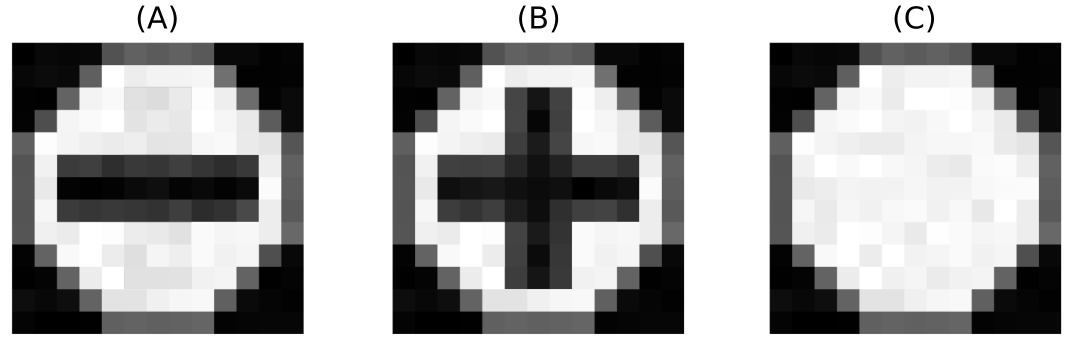
\includegraphics[height=150px]{7.multiatlas/img/phantoms.png}
    \caption{Phantoms created to test how our technique weights the votes.
             (A) Only one tract in the white matter (B) Two tracts crossing. (C) No tracts, free diffusion.}
    \label{fig:pha_exp_1}
\end{figure*}

\subsubsection{Fiber Orientation Density Function from Tractography.}
A tract can be described as a set of streamlines, were a streamline is a
discretrized 3-dimensional curve. Assuming that a streamline doesn't have sharp
turns, we can estimate its directionality within a voxel by looking at its
entry and exit points (Fig. \ref{fig:weighted_diffusion} A). Repeating this for each streamline
on a tract, we obtain a set of directional vectors, representing the directionality
of the tract within the voxel. A fiber ODF can be estimated from this set of
vectors by means of directional statistics. In this work, we use the
Angular Central Gaussian Distribution~\cite{Mardia1999} (ACGD). The ACGD models
antipodal symmetric directional data, and has close forms to estimate its
parameters, making it both suitable and easy to estimate the directionality of
a tract in a voxel~\cite{Mardia1999}.

   
% Since we also want to estimate directionality from tracts, we introduce the concept of acgd
\subsubsection{Label Fusion Weighted by Diffusion}
Majority Voting (Eq. \ref{eq:mvoting}) decides the label of a voxel based on
how many subjects 'vote' for it. Given that we are inferring brain pathways,
we want to introduce a weight that denotes how much the voted tract resembles
the target's diffusion data: 

\begin{equation}
\label{eq:mvoting_weighted}
\hat L(x) = \argmax_{l \in labels} \sum_{s\in S} p(L(x) = l ; L_s(x)) p(D(x) ; D_{sl}(x)).
\end{equation}

In our segmentation scheme, the term $p(L(x) = l ; L_s(x))$ is modeled as in
the voting scheme (eq. \ref{eq:mvoting}). Our second term, $p(D(x) | D_{sl}(x))$
express the probability of seeing the diffusion of our target subject ($D(x)$)
on voxel $x$, given the diffusion of subject $s$ generated by tract $l$ on
the same voxel ($D_{sl}(x)$). Since registering DWIs is complicated~\cite{ODonnell2017},
we want to avoid it. Knowing that water particles in the brain diffuse along
tracts, we can estimate $D_{sl}(x)$ by computing the fODF of the registered tract
$l$. At the same time, we can characterize $D(x)$ with the fODF computed from
the diffusion of the target subject. Now, we want to reflect how much the fODF of
our target subject's diffusion resembles the fODF of the voted tract on a voxel.
We do so by modeling $p(D(x) ; D_{sl}(x))$ as:

\begin{equation}
\label{eq:inner_odf}
\begin{aligned}
    p(D(x) ; D_{sl}(x)) = 
    \begin{cases}
        <F(x), F_{sl}(x)>,& \text{if } L_s(x) = l,\\
                        & \text{and } l \neq 0 \\
        <F(x), U>,& \text{if } L_s(x) = 0 \\
        0,& \text{otherwise}
    \end{cases} \\
    \text{where} \\
    <F(x),F(x)> = 1,\\ < F_{sl}(x), F_{sl}(x)>=1.
\end{aligned}
\end{equation}

In our model, $F(x)$ is the fiber ODF on voxel $x$ estimated from the diffusion
of the target by means of CSD. It's normalized in such a way that the inner
product with itself results in 1. $F_{sl}(x)$ is the fiber ODF of the tract $l$
registered from subject $s$, estimated by means of ACGD. $U$ is a uniformly
distributed fiber ODF, this is the diffusion assumed for either the label 
no-tract, representing the background or a gray matter structure.
By computing the inner product between normalized ODFs, we can estimate how much
they look alike. This allow us to weight the votes of each subject, while
accounting for the white-matter structure of the voting and target subjects.

\section{Experiments and Results}
In section \ref{sec:methods} we presented how to add diffusion information to
Majority Voting (Eq. \ref{eq:mvoting_weighted}). This allow us to weight the
vote for a tract by how much the diffusion of the target supports it. Now, we present
experiments both in synthetic data and subjects from the Human Connectome 
Project (HCP). We start by assessing that the computed weights correctly reflect
the diffusion information in DWI phantoms. Then, we proceed to infer the location
of white-matter pathways in subjects of the HCP, and compare them with their
truth shape. Finally, we simulate lesions in the white-matter and test how our
method behaves in their presence.

\subsection{Data and Preprocessing}
We created three types of diffusion weighted image phantoms using Phantomas~\cite{Caruyer2014}.
The first phantom possess only one tract, traveling from one side to the other of the
image horizontally (Fig. \ref{fig:pha_exp_1} A). The second possess two crossing tracts,
forming a 90 degrees angle between them (Fig. \ref{fig:pha_exp_1} B). The last, has no
fibers, and represents isotropic diffusion (Fig. \ref{fig:pha_exp_1} C). From
each one of them, we generated 31 DWIs. All the DWIs were generated using a
Signal to Noise Ratio of 20, and a resolution of $1mm$ per voxel. The final
images are 3-dimensional matrices, with 10 voxels in each dimension. Having
such small images, allows us to test how our label fusion technique behaves
on a controlled environment.

To test our technique in more realistic scenarios, we randomly selected 10 subjects
from the HCP500 dataset from the Human Connectome Project. For each subject,
we computed whole-brain tractography using each voxel in the white-matter as
a seed and simulating 8 particles per seed~\cite{Garyfallidis2014}. We extracted
the main tracts 4 main tracts from the left hemisphere using
the implementation of the white-matter query language (WMQL)~\cite{Wassermann2016}.
For each subject we computed non linear registrations to the rest using as
reference their T1w images~\cite{Jenkinson2012}. Using the resulting warp
transformations, we registered the tracts between every pair of subjects.

We estimated fibet ODFs in the voxels of each phantom DWIs, and in the DWI data
of the HCP subjects by means of CSD in Dipy~\cite{Garyfallidis2014}. The ODFs were
discretrize on a sphere with $n=100$ vertices. A uniform distribution over the sphere
was created by assigning to each vertex the value $\sqrt(n)/n$, making $<U, U> = 1$.

\begin{figure*}[t]
    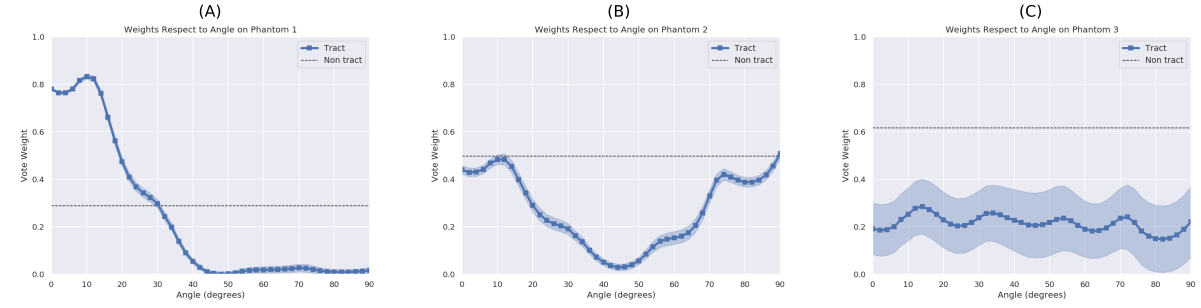
\includegraphics[width=\textwidth]{7.multiatlas/img/weights.png}
    \caption{We started with an horizontal tract and start rotating it. We computed
             the weight a subject would get when voting for the tract. 
             (A) Weights in phantom A (B) Weights in phantom B (C) in C.}
    \label{fig:weights}
\end{figure*} 

\subsection{Assessing the Correctness of Voting Weights in Synthetic Data}
In order to study how the tract's directionality influences its vote weight,
we started by reconstructing the tract present in the first phantom (Fig. \ref{fig:pha_exp_1} A).
For this, we took one of the 31 generated DWIs, and computed 1000 streamlines by
means of probabilistic tracking from the voxels in which the tract passes.

In the DWIs generated from the first phantom, the reconstructed tract is the one
that should generate the highest weight. At the same time, any change in its
directionality, should decrease the received weight. To assess this was happening,
we computed weights in 30 DWIs for the reconstructed tract, and for planar
rotations of it around the central voxel. Figure \ref{fig:weights} A shows the
obtained weights on the first phantom. Effectively, the weight starts to rapidly
decrease as the angle increments and the directionality of the tract moves away
from that of the diffusion. Figure \ref{fig:weights} B shows the weights obtained
when computing weights of the reconstructed tract in 30 DWIs derived from the
second phantom (Fig. \ref{fig:pha_exp_1} B), which have a crossing of fibers in
the central voxel. In this case, the weight is higher when the reconstructed tract
aligns with one of the crossing fibers (at 0 degrees or 90 degrees), while rapidly
decaying in between them. Finally, figure \ref{fig:weights} C shows the weights
when using 30 DWIs with isotropic diffusion (Fig. \ref{fig:pha_exp_1} C). In this
case, the weight is always low, driven by the discrepancy between the
directionality of the tract and the free diffusion present in the DWIs.

To assess that the proposed model is not overweighting tracts, we also computed
the weight that a 'non-tract' label would receive in each of the phantoms. As
explained in section \ref{sec:methods}, equation \ref{eq:inner_odf}, when a
subject is voting for a non-tract label, a uniform fiber ODF is compared against
the diffusion fODF. Figure \ref{fig:pha_exp_1} A, B, and C show the weight
obtained in the central voxel when a subject is voting for the label 'no-tract'.
In figure \ref{fig:pha_exp_1} A, we can see that the
weight of 'no-tract' is low, specially when compared with the high weight
of the correctly aligned tracts (low angle rotations). This is driven by the
highly directional underlying diffusion data of the phantom. 
Figure \ref{fig:pha_exp_1} B shows that the weight of a 'no-tract' vote is
similar to that of an aligned tract. Finally, figure \ref{fig:pha_exp_1} C
shows always a higher weight for the 'non-tract' than for any tract, consistent
with the isotropic diffusion of our third phantom.

\subsubsection{Inferring Tracts in Human Connectome Project Subjects}
To validate our technique in a more realistic but yet controlled scenario, we
inferred single tracts in the HCP subjects. We selected the following tracts to
work with: inferior part of the Superior Longitudinal Fasciculus (SLF1),
Inferior Longitudinal Fasciculus (ILF), middle part of the
Corpus Callosum (CC2), and External Capsule (EC). These four tracts provide
a fair diversity of directionality, shape, and position in the brain.

For each tract we performed a leave-one-out cross-validation. At each step, we
inferred the tract of one subject from the registered tracts of the others
using both Majority Voting and our technique. Using as 'ground truth' the
target's bundle computed by means of tractography and WMQL, we quantified the
performance of both techniques. In particular, we computed their confusion matrix.
A confusion matrix is a matrix $M \in \R^(2\times2)$, where each the entry $M_{ij}$
represents the number of times the label in the ground truth was i and the
technique labeled j. Finally, we computed the sensitivity, and precision on
each confusion matrix~\cite{Kuhn2013}. Sensitivity measures the proportion of voxels
in the ground-truth tract that were 'discovered'. Precision measures the proportion
of voxels that were correctly labeled, over all the labeled voxels. Table 1 shows
the results obtained for each technique and tract. In all of the tracts, our
technique achieves a lower sensitivity than Majority Voting. This means that
we label a smaller portion of the ground-truth bundle. On the other hand,
our diffusion weighted label-fusion always achieve a higher precision. This
is, if we only look at the labels created by the techniques, our technique
has the highest proportion of correct ones. Another way to phrase it is, our
technique has a lower number of false positives.
Therefore, our technique is discovering less voxels, but those which are labeled
can be trusted more.

\begin{figure*}[t]
    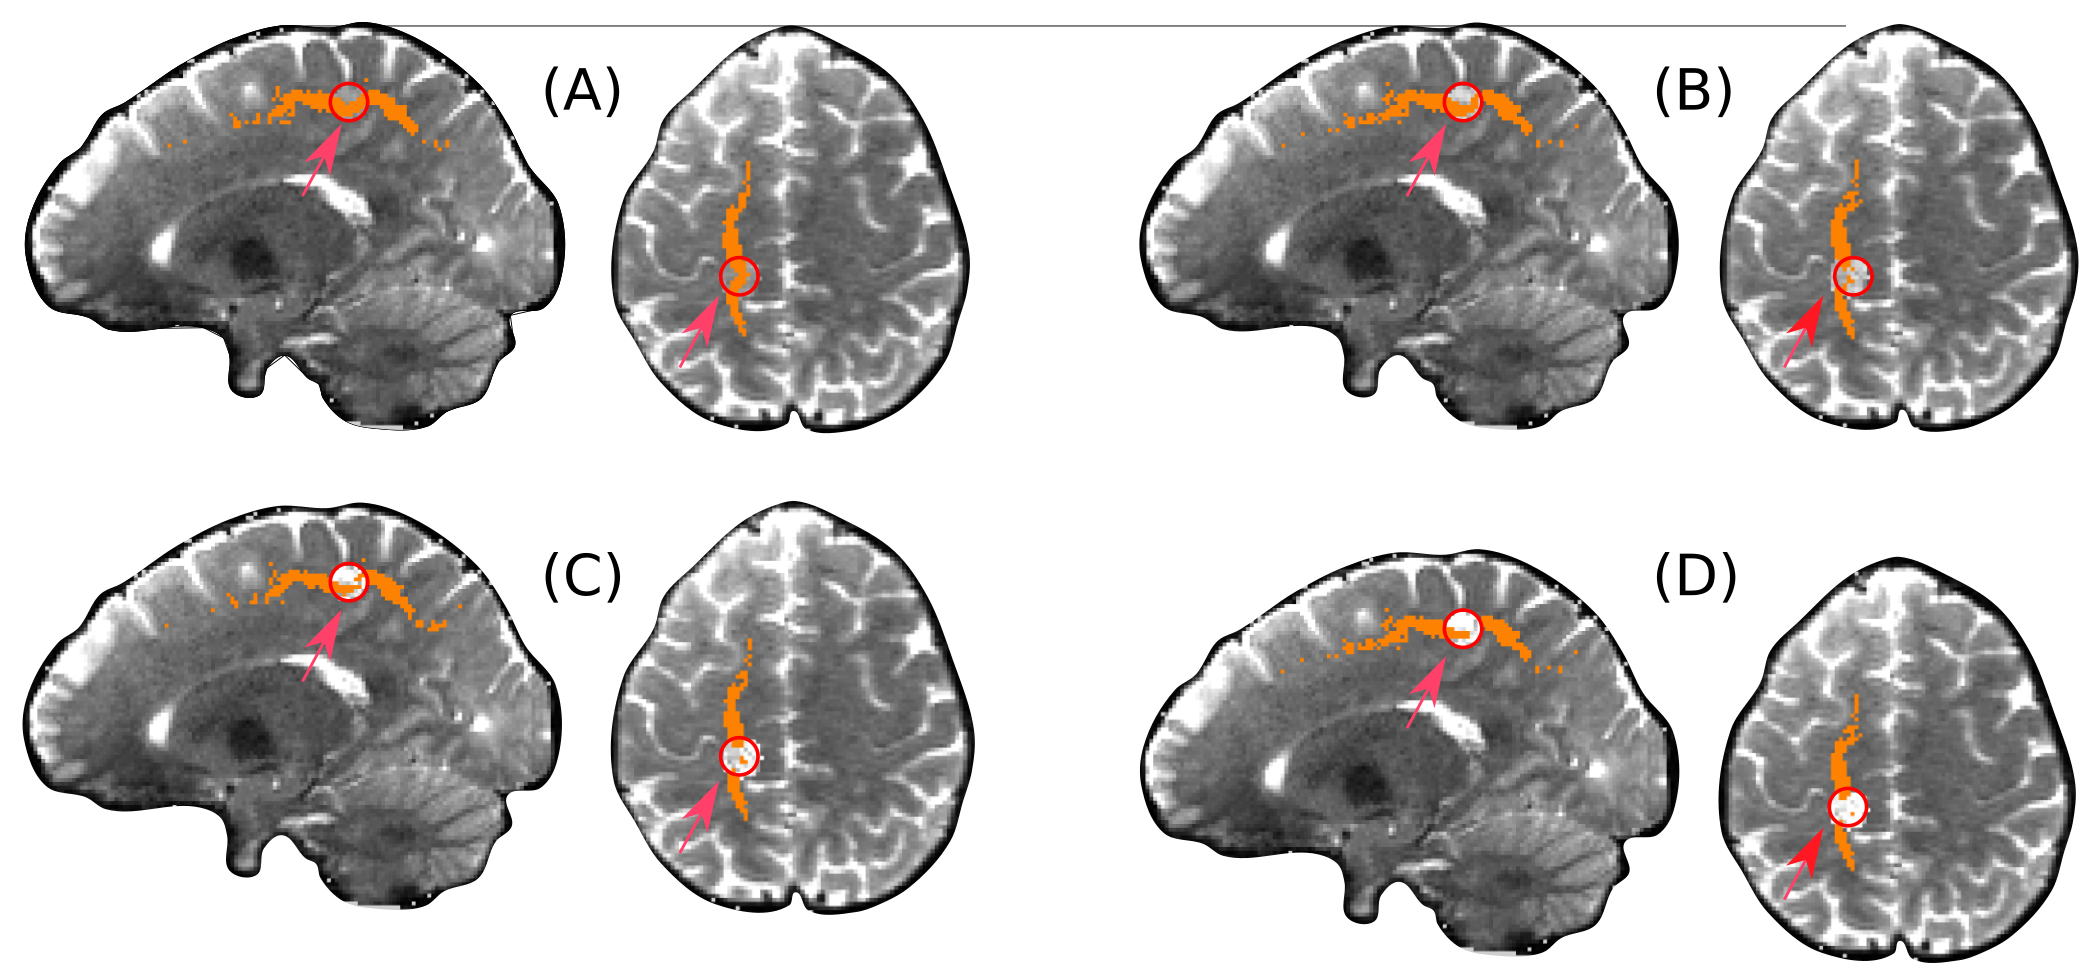
\includegraphics[width=\textwidth]{7.multiatlas/img/pathology.png}
    \caption{Test of tract retrieval when a lesion (red circle) is present.
             Lesions were simulated by mixing the signal with isotropic data,
             following eq. \ref{eq:mixing}. (A) $\alpha=0.2$
             (B) $\alpha=0.5$ (C) $\alpha=0.75$ (D) $\alpha=1$. Our technique
             labels less voxels as alpha increases.}
    \label{fig:labeling}
\end{figure*}

\subsubsection{Inferring Tracts in the Presence of Simulated Lesions}
To test how our technique behaves on an injured brain, we simulated
lesions at different degrees of severity in the white matter of one of our subjects.
Given that some brain lesions directly affect FA~\cite{Schonberg2006, Huisman2009},
we simulated lesions by adding isotropic signal to a set of voxels, therefore
lowering their FA. We targeted the SLF bundle, in order to compare how the labeling
changes with lesion of different degrees. We did so by selecting a spherical region
of $4mm$ where the SIF passes by, and mixing the diffusion signal there with signal
from the ventricles. Since the ventricles are regions filled with cerebrospinal
fluid (CSF), their diffusion is approximately isotropic. In particular, for each
voxel $x$ in the lesioned region, we chose a voxel $v$ in the ventricle and mix
their signals ($S(\cdot)$) as follows:

\begin{equation}
    \label{eq:mixing}
S(x) = S(x)(1-\alpha) + S(v)\alpha, \alpha \in [0,1],
\end{equation}

where $\alpha$ manages the severity of the lesion. In this case, $\alpha=0$
represents healthy tissue, and $alpha=1$ represents a total disruption of
the white-matter, resulting in pure isotropic diffusion. Figure \ref{fig:}
shows that, at higher alpha (lower FA), less voxels are labeled within the lesion.
This is a good behaviour, since by lowering the FA we make the diffusion more
isotropic, loosing the underlying tract. In particular, for $\alpha=1$, the
diffusion is completely isotropic, meaning that there's no tract, therefore,
it's correct to not label it. Since our technique still labels the surroundings
of the pathology, it allows to correctly identify the affected tract.

\subsection{Discussion}
In this work we presented a label-fusion techniques to infer white-matter
structures in the brain. An advantage of label-fusion techniques is that
they can achieve accurate segmentations even when the inference is
made from few subjects~\cite{Asman2013}. In particular, our technique allows to
infer white-matter pathways without the need of tracking. This is of specially
importance in the presence of brain pathologies that show no deformations. In the case of having
deformations, then the registration between subjects, in which label-fusion
techniques heavily rely, becomes hard. The main contribution of this work
was to add diffusion information in the process of label-fusion. Given that fiber
bundles constrains the diffusion of
water particles in the brain, our technique uses diffusion information to improve
Majority Voting~\cite{Xu1992}. More specifically, we weight each vote based on how
the voted pathway is supported by the target's diffusion data. In this way, voted
pathways that better resemble the white matter of the target subject obtain a 
higher weight. The weights come from comaring how much the diffusion fODF of our
target subject's resembles the fODF of the voted tract on a voxel. In this way, we
can compare the white-matter structure of our target subject with that of the voting
subject, without having to register DWIs. Adding diffusion weights to Majority Voting,
allowed us to profit of its robustness while improving the labeling of white-matter
bundles, as shown by our results in synthetic data and subjects from the Human
Connectome Project.

\subsubsection{Our Technique Creates Weights Consistent With the Underlying
               Diffusion Data.}
In order to study how the tract's directionality influences its vote weight,
we created three different phantoms, and derived DWIs from them. This allowed us to
create a controlled environment, in which to study how the directionality
of a tract affects its vote weight. Since the variability in the weights can
come from changes on the directionality or the tract, we generated many DWIs
for each phantom. At the same time, we computed weights for tracts in different
directions. Figure \ref{fig:pha_exp_1} shows the weights obtained on a phantom
with a single bundle. The weights show that tracts with a directionality
similar to the underlying diffusion get higher votes. But, when the alignment
start to decrees, also does the weight. In particular, when the directions
differ by more than 20 degrees, the weight starts to drop rapidly, falling bellow the weight of the
'non-tract' label.
The Figure \ref{fig:pha_exp_1} B shows that, in the presence of crossing fibers
in the DWI, tracts aligned with a crossing fibers get the highest weights.
It is important to notice that the highest weights are similar to those of the
'non-label' votes. This means, that tracts roughly aligned with one of the
crossing fibers will compete with equal weights against the 'non-label' structures.
Finally, Figure \ref{fig:pha_exp_1} C shows that, when there's no underlying
white-matter structure in the DWI image,
then the label 'no-tract' is the one that receives the highest weight. These
results show that our technique is able to correctly weight each label based
on diffusion directionality.

\subsubsection{Our Technique Incurred in a Trade-off Between the Amount of
               Labeled Voxels and Their Correctness.}
To test our technique in realistic data, we registered tracts between different
subjects of the HCP. Using these registered tracts, we inferred the position
of individual tracts in each subject. Table \ref{table:sensitivity} shows that
in each inferred tract, our technique achieved a lower sensitivity but a higher
precision. In fact, the precision, except for the External Capsule, is always
higher than 0.7. This means that our technique was able to discover less voxels
belonging to the tracts, but at least 70\% of those labeled are correct. Another
way to phrase this is that our techniques presents less false positives at the
cost of more false negatives, making it more conservative than Majority Voting.

\subsubsection{Our Technique Behaves Correctly in the Presence of Pathologies}

We further characterized the behaviour of our technique by simulating lesions
in the white-matter of a HCP subject. In particular, we defined a spherical region
on the path of the Superior Longitudinal Fasciculus, and increased its
Fractional Anisotropy until achieving isotropic diffusion. By doing so, we
We simulated lesions in the brain of a subject for two types of pathologies:
edema-like pathology, and tumor-like with no tract displacement. As explained
in the introductions, these pathologies are characterize by a decreased FA inside
the lesion, but do not deform the white-matter around it. Figure \ref{fig:labeling}
shows that our technique labels less voxels as the FA becomes higher on the
region. This is a correct behaviour, since the more isotropic is the region,
the less it is related to a white-matter tract. However, since our technique
is still able to label the surroundings of the lesion, we can still identify
the affected tract. It is important to notice that the simulated lesions do not
account for mass-effect, this is, white matter deformations. Such pathologies
are difficult to simulate and study, since the process of registration from
healthy subjects to the patient has to be fined tuned manually . 

\subsection{Conclusions}
In this chapter we presented a labeling fusion technique that relies on dMRI
data to infer the localization of white-matter tracts. The results show that
our technique is more conservative than the voting rule, which is desired when
studying pathologies, at the cost of having more false negatives.

\begin{table*}[t]
    \label{table:sensitivity}
\centering
    \caption{Sensitivity and precision of our proposed
             method (Weighted) and Majority Voting (Majority) when inferring single
             bundles in 9 subjects. The inferred bundles are: Superior Longitudinal
             Fasciculus (SLF), Inferior Longitudinal Fasciculus (ILF), Corpus
             Callosum (CC), and the External Capsule (EC).}
\label{my-label}
\begin{tabular}{|l||c|c||c|c||c|c||c|c|}
\hline
 & \multicolumn{2}{c|}{SLF} & \multicolumn{2}{c||}{ILF} & \multicolumn{2}{|c||}{CC} & \multicolumn{2}{|c|}{EC}\\ 
 \hline
            &  Weighted & Majority & Weighted & Majority & Weighted & Majority & Weighted & Majority \\
  \hline
Sensitivity & 0.19\rpm0.04 & \bf{0.30}\rpm0.05 & 0.33\rpm0.02 & \bf{0.47}\rpm0.07 & 0.53\rpm0.04 & \bf{0.64}\rpm0.09 & 0.06\rpm0.02 & \bf{0.27}\rpm0.20 \\
  \hline                                                                                                                               
Precision   & \bf{0.70}\rpm0.11 & 0.58\rpm0.10 & \bf{0.74}\rpm0.05 & 0.41\rpm0.20 & \bf{0.91}\rpm0.15 & 0.82\rpm0.17 & \bf{0.42}\rpm0.20 & 0.31\rpm0.13 \\
\hline
\end{tabular}
\end{table*}

\chapterbib
